\chapter{Methodology}
\label{chap:methodology}
This chapter presents the methodology for implementing and evaluating a Model Context Protocol (MCP) server designed for ASUS routers. The primary focus is on developing a system that enables AI assistants to securely access and control router functionality through structured tools, measuring its performance, and validating its functionality through automated testing.
An overview of the methods undertaken is presented in Figure \ref{fig:methodology-overview}. This illustrates the systematic workflow from initial setup through implementation and evaluation phases, addressing server implementation, performance assessment, and validation testing.
\begin{figure}[h]
\centering
% [PLACEHOLDER IMAGE: Methodology workflow diagram showing the systematic process flow from initial setup through implementation and evaluation phases, including hardware configuration, MCP server development, tool implementation, and performance testing stages]
\caption{Overview of the Methodology Workflow}
\label{fig:methodology-overview}
\end{figure}
\section{Implementation Environment and Artifact Description}
The technical implementation of the MCP server was conducted within a specific hardware and software environment designed to replicate a typical home or small office network setup.
\subsection{Hardware Artifact}
The ASUS RT-AX57 Go router was selected as the hardware artifact for this study due to its modern Wi-Fi 6 capabilities, compact form factor, and representative feature set running the standard ASUSWRT firmware, making it a suitable testbed for developing and evaluating the MCP server in a realistic context. The router was configured with firmware version 3.0.0.6.10256040, which includes recent security enhancements and is compatible with the asusrouter library. This model runs stock ASUSWRT firmware, as Merlin firmware is not available for the RT-AX57 Go.
\subsection{Software Environment}
Key Python Libraries used in the implementation:
\begin{enumerate}
\item Python 3.11: The minimum required Python version for the asusrouter library;
\item asusrouter vX.Y.Z: The specific version of the asusrouter Python API wrapper used for interacting with the router. This library communicates with the router using HTTP(S) protocols and is built for asynchronous operations using asyncio;
\item fastmcp vA.B.C: The version of the fastmcp framework used to build the MCP server. fastmcp simplifies the creation of MCP servers by handling the underlying protocol complexities; and
\item aiohttp vP.Q.R: An asynchronous HTTP client/server framework for handling the asynchronous network communication with the router.
\end{enumerate}
\subsection{MCP Server Architecture}
The MCP server's architecture is designed around the fastmcp framework, exposing router functionalities as callable tools for an AI assistant. It operates as a service that listens for incoming MCP requests, processes them by calling the appropriate asusrouter functions, and returns the results in the MCP format. Security considerations, such as using HTTPS for communication with the router and implementing input validation within the tools, are integrated into the design.
\section{MCP Tool Development and Mapping}
The process of developing the MCP tools involved identifying relevant ASUS router functionalities accessible via the asusrouter library and mapping them to standardized Model Context Protocol tools.
\begin{figure}
\centering
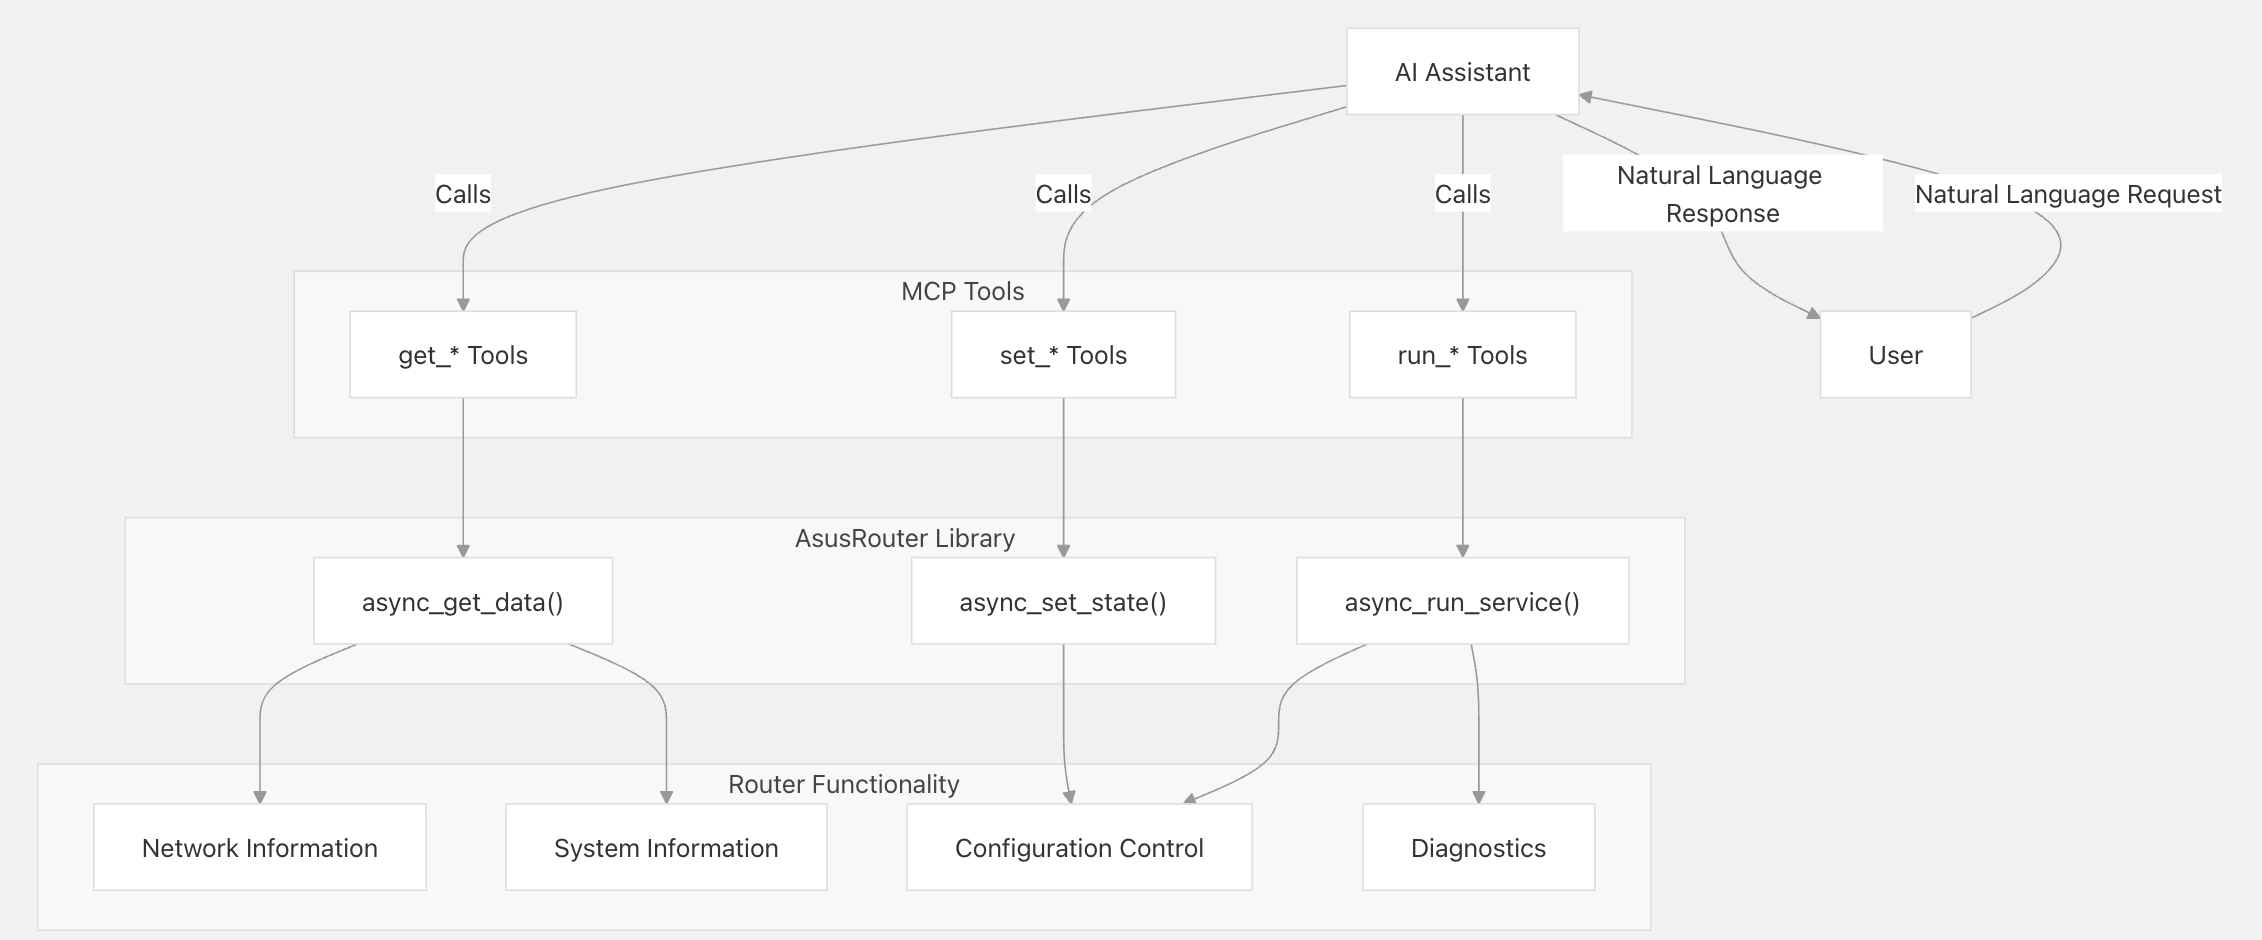
\includegraphics[width=1\linewidth]{architecture.png}
\caption{MCP Tool Mapping Process and Architecture}
\label{fig:mcp-mapping}
\end{figure}
\subsection{asusrouter Library}
The asusrouter library provides an asynchronous API wrapper that abstracts the complexities of direct HTTP requests to the router's web interface backend.
\begin{enumerate}
\item While there is no official documented API for ASUS routers, the asusrouter library leverages reverse engineering of the httpd daemon to interact with the router;
\item This library supports various functionalities, including monitoring connected devices, CPU/RAM usage, guest WLAN, and network traffic; and
\item Compatibility is dependent on the router's firmware version.
\end{enumerate}
\subsection{Tool Selection and Implementation}
The selection of specific tools was guided by the objective of enabling an AI assistant to perform common network management and diagnostic tasks. The implemented tools fall into four main categories: Network Information, System Information, Configuration Control, and Diagnostics.
The implementation process followed these key steps:
\begin{enumerate}
\item For each selected functionality, a corresponding Python function was created within server.py, decorated with @mcp.tool() to make it discoverable and callable by an MCP client;
\item Inside each tool function, the appropriate asusrouter method or data enum is called to interact with the router;
\item The implementation ensured that the MCP tools correctly awaited the results of the asynchronous calls from the asusrouter library; and
\item Error handling was integrated to manage potential issues such as connection errors, timeouts, or unexpected responses from the router API. This includes anticipating rate limit errors and implementing strategies like exponential backoff or caching where appropriate.
\end{enumerate}
\subsection{Mapping to MCP}
The mapping process addressed the challenges of abstracting complex network tasks into atomic, AI-callable tools:
\begin{enumerate}
\item Each tool was designed to perform a single, well-defined action or retrieve a specific piece of information; and
\item The docstrings for each tool were carefully written to provide clear descriptions, parameters, and return values, adhering to the MCP specification.
\end{enumerate}
A comprehensive summary of the MCP tool implementation is provided in Appendix \ref{app:mcp_tools}.
\section{Technical Evaluation Methodology}
This section describes the procedures for quantitatively measuring the technical performance metrics of the MCP server and its tools, focusing on response time, command accuracy, error rates, and system stability.
\subsection{Performance Metrics}
The key performance indicators (KPIs) for the MCP server's technical evaluation are:
\begin{enumerate}
\item \textbf{Response Time:} The duration between an MCP request being sent to the server and the corresponding response being received, measured for each implemented tool call;
\item \textbf{Command Accuracy:} The percentage of configuration or action-oriented tool calls that successfully achieve the intended state change on the router;
\item \textbf{Error Rates:} The frequency of failed tool calls, categorized by error type (e.g., connection errors, API errors, validation errors, rate limit errors); and
\item \textbf{System Stability:} The ability of the MCP server and the router API to maintain consistent performance and availability under load, including monitoring the router's CPU and memory usage.
\end{enumerate}
\subsection{Test Cases}
A comprehensive set of test cases was designed to cover the functionality of each implemented MCP tool:
\begin{enumerate}
\item \textbf{Read Operations:} Repeated calls to "get" tools to measure response time and consistency of data retrieval;
\item \textbf{Write Operations:} Calls to "set" or "run" tools to measure accuracy and the time taken for the router to apply changes;
\item \textbf{Sequential Operations:} Chains of tool calls that simulate a typical user interaction workflow; and
\item \textbf{Error Condition Testing:} Test cases designed to deliberately trigger known or anticipated error conditions.
\end{enumerate}
The exact test prompts used for each tool are detailed in Appendix \ref{app:mcp_test_cases}.
\subsection{Network Conditions and Load Simulation}
To evaluate performance under realistic conditions, the testing environment simulates varying network loads and device counts:
\begin{enumerate}
\item \textbf{Varying Device Counts:} The number of connected devices is varied to assess the impact on the router's API responsiveness; and
\item \textbf{Concurrent API Requests:} The test harness issues multiple concurrent MCP tool requests to simulate scenarios where an AI assistant might be performing several tasks simultaneously.
\end{enumerate}
\subsection{Verification of Configuration Changes}
A critical aspect of assessing command accuracy is verifying that configuration changes requested via the MCP tools are correctly applied by the router. For each configuration task performed via an MCP tool, a subsequent call to a relevant "get" tool is made to retrieve and verify the current state of the configuration.
\subsection{Automated Testing Framework}
An automated testing framework using Python scripts orchestrates the test cases, simulates network conditions, executes MCP tool calls, collects data, and performs initial analysis. The test scripts interact directly with the MCP server's API.
\section{Data Collection and Analysis Procedures}
This section delineates the methodology for collecting and analyzing quantitative data generated during the technical evaluation.
\subsection{Data Collection Methodology}
The automated testing framework serves as the primary instrument for quantitative data acquisition. The following data points are systematically recorded:
\begin{enumerate}
\item \textbf{Temporal Parameters:} Request and response timestamps
\item \textbf{Request Specifications:} MCP tool identifier and input parameters
\item \textbf{Response Characteristics:} Complete response payload and error typology (when applicable)
\item \textbf{Verification Metrics:} For configuration control tests, verification outcomes including success/failure indicators
\end{enumerate}
All data are preserved in structured formats (JSON or relational database) to facilitate subsequent analytical procedures.
\subsection{Analytical Framework}
The quantitative data undergo analysis through descriptive statistics and systematic error pattern evaluation:
\subsubsection{Performance Metric Evaluation}
\begin{enumerate}
\item \textbf{Latency Analysis:} Calculation of central tendency measures and dispersion indicators for response times across all implemented tools under varied conditions
\item \textbf{Throughput Assessment:} Quantification of successful tool request processing rates under controlled load conditions

\item \textbf{Error Frequency Analysis:} Computation of aggregate and tool-specific error rates, categorized by error typology

\item \textbf{Resource Utilization Profiling:} Correlation analysis between server/router resource consumption metrics and test execution phases
\end{enumerate}
\subsubsection{Command Accuracy Evaluation}
Quantitative assessment of configuration application success rates based on verification outcomes, with particular focus on identifying specific configuration parameters exhibiting reduced reliability.
\subsubsection{Error Pattern Examination}
Systematic classification and frequency analysis of logged errors to establish common failure modes and their precipitating conditions, including investigation of rate-limiting occurrences and API-specific error patterns.
\section{Conclusion}
This chapter has detailed the methodology for developing and evaluating an MCP server for ASUS routers. The approach encompasses the technical implementation, performance measurement, and validation testing required to meet the research objectives:
\begin{enumerate}
\item The implementation environment, MCP server architecture, and tool development process provide a framework for developing a robust MCP server with proper error handling and security controls;
\item The technical evaluation methodology, with its focus on performance metrics, test cases, and network conditions, establishes procedures for measuring response time, command accuracy, error rates, and system stability; and
\item The automated testing framework, verification procedures, and error pattern examination support the verification and validation of the technical functionality through comprehensive testing under various conditions.
\end{enumerate}
The results of applying this methodology will provide empirical evidence regarding the technical feasibility and performance characteristics of using the Model Context Protocol to bridge AI assistants with network hardware.